\documentclass{beamer}

% Tema limpio y moderno
\usetheme{Madrid} % Puedes probar: Warsaw, CambridgeUS, Frankfurt, Boadilla, etc.
\usecolortheme{default}

% Información del documento
\title{Modelo predictivo para la gestión de inventarios en tiendas de abarrotes en Puno usando ARx y programación lineal entera}
%\subtitle{Subtítulo opcional}
\author{
Caceres Tacora Lizbeth Estefany\\
Butron Maquera Tania Karin\\
Paredes Cuaguila Fiorella Yaneth\\
Mamani Mena Ronaldo Carlos\\
}
\institute{Métodos de Optimización}
\date{\today}
% Barras superior e inferior
\setbeamertemplate{footline}{
  \leavevmode%
  \hbox{%
  \begin{beamercolorbox}[wd=\paperwidth,ht=2ex,dp=1ex]{author in head/foot}%
    \color{darkceleste}\rule{\paperwidth}{1.5pt}
  \end{beamercolorbox}}%
}
\setbeamertemplate{headline}{
  \leavevmode%
  \hbox{%
  \begin{beamercolorbox}[wd=\paperwidth,ht=2ex,dp=1ex]{author in head/foot}%
    \color{darkceleste}\rule{\paperwidth}{1.5pt}
  \end{beamercolorbox}}%
}
\begin{document}

% Portada
\begin{frame}
    \titlepage
\end{frame}

\begin{frame}{Introducción}
    \vspace{-0.2cm} % Subimos el contenido

    \textbf{Punto clave 1}\\
    Las tiendas de abarrotes en Puno, especialmente cerca de la UNA, operan sin herramientas técnicas, lo que genera pérdidas o desabastecimiento.

    \vspace{0.4cm}
    \textbf{Punto clave 2}\\
    Se aplicó un modelo ARx ARIMA con datos de 72 semanas. Se analizaron 52 semanas para identificar patrones y predecir demanda de productos básicos.
\end{frame}

% Diapositiva 2
\begin{frame}{Introducción}
    \vspace{-0.2cm} % También subimos esta

    \textbf{Objetivo de la presentación}\\
    Mostrar cómo la estadística y programación pueden mejorar las decisiones de compra en pequeños negocios, optimizando el inventario y reduciendo pérdidas.
\end{frame}
% Sección 2--- PARTE DE FIORELLA------------------------
% Diapositiva: Base de Datos
\begin{frame}{Base de Datos}
  \vspace{0.3cm}
  \textbf{En este estudio, se utilizó un conjunto de datos sintéticos de ventas semanales de 6 productos de consumo diario en tiendas de vecindario.}
  \vspace{0.5cm}
  \begin{table}[]
    \centering
    \caption{Productos seleccionados}
    \renewcommand{\arraystretch}{1.3}
    \begin{tabular}{|c|l|}
    \hline
    Producto 1 & Pan \\ \hline
    Producto 2 & Pollo \\ \hline
    Producto 3 & Arroz \\ \hline
    Producto 4 & Huevo \\ \hline
    Producto 5 & Detergente \\ \hline
    Producto 6 & Shampoo \\ \hline
    \end{tabular}
  \end{table}
\end{frame}

% Diapositiva: Segmentación del Dataset
\begin{frame}{Segmentación del Dataset}
  \vspace{0.3cm}
  \textbf{La demanda de cada producto por semana se muestrea durante un periodo de 78 semanas.}
  \vspace{0.5cm}
  \begin{table}[]
    \centering
    \caption{Segmentación en subconjuntos}
    \renewcommand{\arraystretch}{1.3}
    \begin{tabular}{|l|c|c|}
    \hline
    Conjunto & Semanas Incluidas & N° de Semanas \\ \hline
    Entrenamiento & 1 – 56 & 56 \\ \hline
    Validación & 57 – 78 & 22 \\ \hline
    \end{tabular}
  \end{table}
\end{frame}

% Diapositiva: Variables Exógenas
\begin{frame}{Variables Exógenas}
  \vspace{0.3cm}
  \textbf{Para cada producto, las ventas de los otros cinco productos actúan como variables exógenas que pueden influir en la demanda.}
  \vspace{0.3cm}
  Esto permite captar efectos de complementariedad o sustitución en la demanda semanal.
\end{frame}

% Diapositiva: Modelado de la Demanda (ARIMAX)
\begin{frame}{Modelado de la Demanda (ARIMAX)}
  \vspace{0.3cm}
  \textbf{El modelo ARIMAX (AutoRegressive Integrated Moving Average with eXogenous variables) constituye una extensión de los modelos ARIMA.}
  \vspace{0.3cm}
  Combina componentes autorregresivos, integrados y de medias móviles con variables exógenas.
\end{frame}

% Diapositiva: Métricas de Desempeño
\begin{frame}{Métricas de Desempeño}
  \vspace{0.3cm}
  \textbf{Para evaluar la precisión de los modelos hemos utilizado:}
  \vspace{0.5cm}
  \begin{table}
      \centering
      \renewcommand{\arraystretch}{1.3}
      \begin{tabular}{|c|c|}
           \hline
           \textbf{Métrica} & \textbf{Descripción} \\ \hline
           MAE & Mean Absolute Error \\ \hline
           RMSE & Root Mean Squared Error \\ \hline
           MAPE & Mean Absolute Percentage Error \\ \hline
      \end{tabular}
      \label{tab:my_label}
  \end{table}
\end{frame}
%----------------------PARTE DE TANIA ----------------------------
\begin{frame}{Resultados del An\'alisis}
\begin{block}{Objetivo}
Predecir la demanda semanal de 6 productos esenciales y optimizar las decisiones de compra bajo una restricci\'on presupuestaria.
\end{block}
\begin{itemize}
    \item Modelo: ARX (AutoRegresivo con variables ex\'ogenas)
    \item Horizonte de predicci\'on: 22 semanas
    \item Datos de entrenamiento: 56 semanas
\end{itemize}
\end{frame}

% --- Diapositiva 2: Predicci\'on de la demanda ---
\begin{frame}{ Predicci\'on de la demanda}
\begin{block}{Modelo ARX}
Se us\'o para estimar la demanda de pan, pollo, arroz, huevo, detergente y shampoo.
\end{block}
\begin{itemize}
    \item M\'etricas evaluadas: MAE, RMSE y MAPE
\end{itemize}
\vspace{0.3cm}
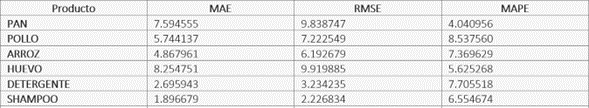
\includegraphics[width=0.75\textwidth]{error.png}
\end{frame}

% --- Diapositiva 3: Resultados visuales de la predicci\'on ---
\begin{frame}{Visualizaci\'on: Predicci\'on vs. Real}
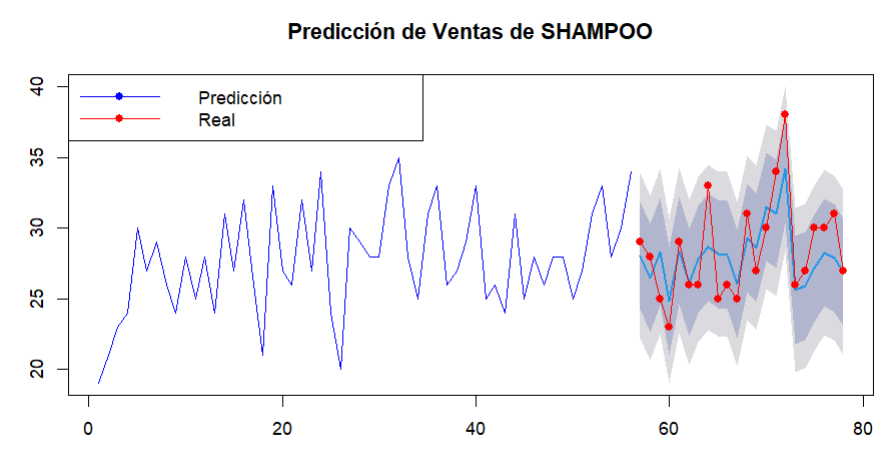
\includegraphics[width=0.8\textwidth]{i1.png}
\end{frame}
\begin{frame}{Visualizaci\'on: Predicci\'on vs. Real}
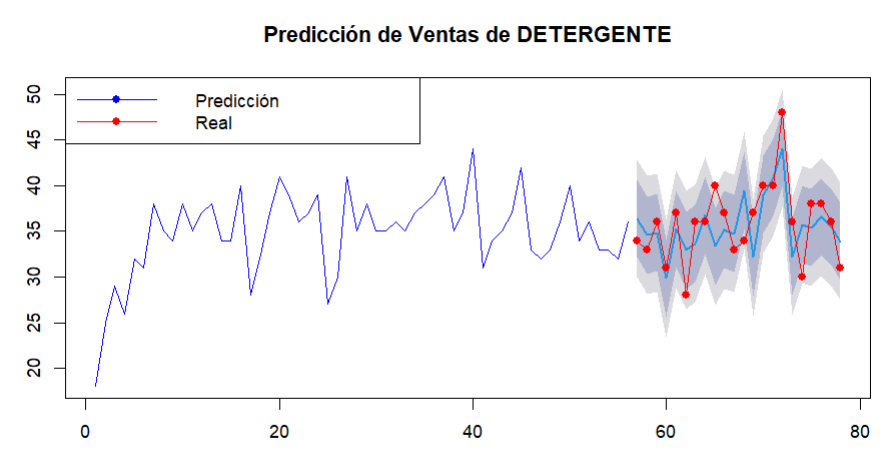
\includegraphics[width=0.8\textwidth]{i2.png}
\end{frame}
\begin{frame}{Visualizaci\'on: Predicci\'on vs. Real}
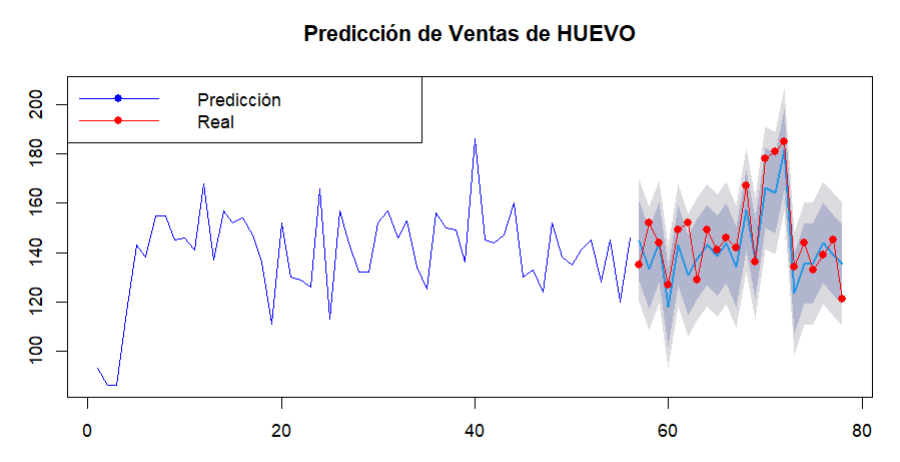
\includegraphics[width=0.8\textwidth]{i3.png}
\end{frame}
\begin{frame}{Visualizaci\'on: Predicci\'on vs. Real}
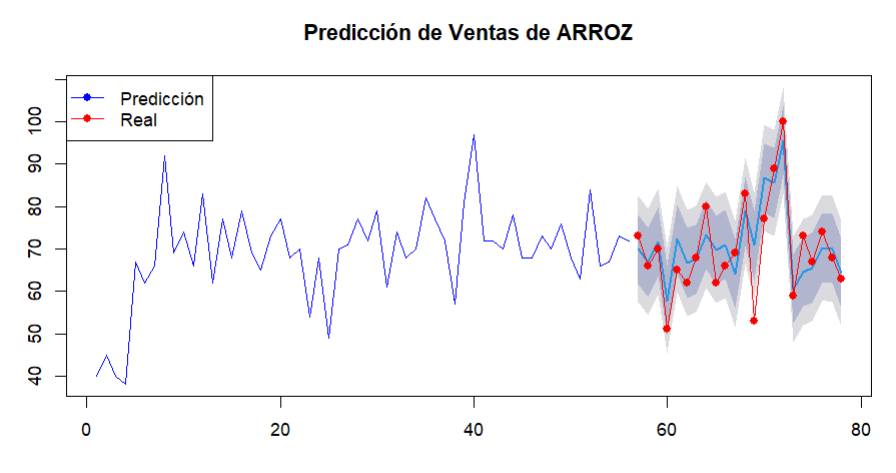
\includegraphics[width=0.8\textwidth]{i4.png}
\end{frame}
\begin{frame}{Visualizaci\'on: Predicci\'on vs. Real}
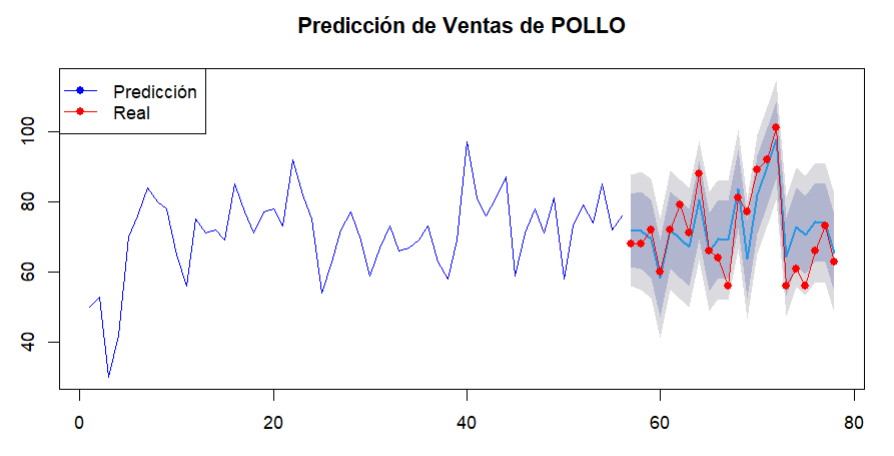
\includegraphics[width=0.8\textwidth]{i5.png}
\end{frame}
\begin{frame}{Visualizaci\'on: Predicci\'on vs. Real}
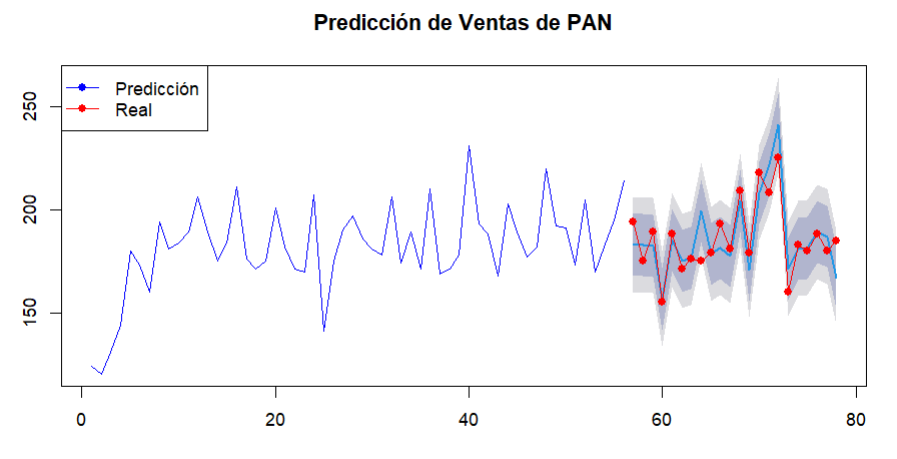
\includegraphics[width=0.8\textwidth]{i6.png}
\end{frame}
% --- Diapositiva 4: Optimizaci\'on de compras ---
\begin{frame}{Optimizaci\'on de decisiones de compra}
\begin{block}{Modelo de Programaci\'on Lineal Entera}
Maximiz\'o la ganancia semanal bajo:
\end{block}
\begin{itemize}
    \item Presupuesto m\'aximo: S/. 500 por semana
    \item L\'imite: no superar la demanda predicha
\end{itemize}
\vspace{0.3cm}
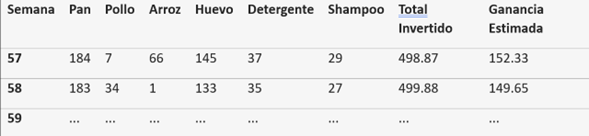
\includegraphics[width=0.75\textwidth]{tablaPRED.png}
\end{frame}

% --- Diapositiva 5: Inversi\'on y ganancia semanal ---
\begin{frame}{An\'alisis visual de los resultados}
\textbf{Inversi\'on y ganancia semanal (semanas 57--78)}
\begin{itemize}
    \item Inversi\'on cercana al l\'imite presupuestario
    \item Ganancia estable: > S/. 150, con picos hasta S/. 190
\end{itemize}
\vspace{0.3cm}
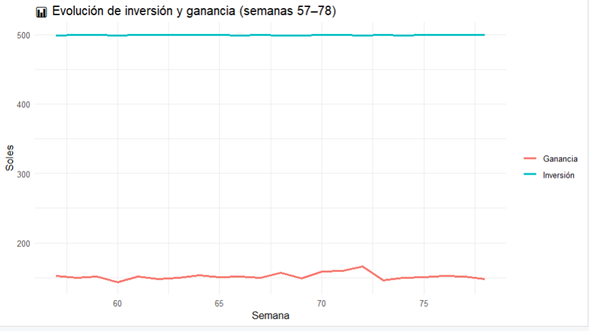
\includegraphics[width=0.75\textwidth]{Imagen3.png}
\end{frame}

% --- Diapositiva 6: Unidades adquiridas ---
\begin{frame}{Evoluci\'on de unidades adquiridas}
\begin{itemize}
    Prioriza lo rentable, reduce lo innecesario, y ajusta cada semana la compra según lo que más conviene
\end{itemize}
\vspace{0.3cm}
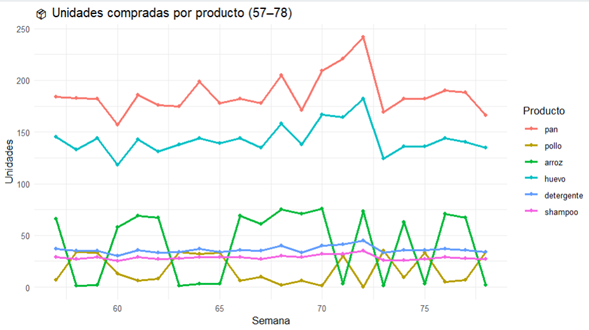
\includegraphics[width=0.8\textwidth]{uproducto1.png}
\end{frame}

\begin{frame}{Hallazgos principales}
\begin{itemize}
    \item Se combinó un modelo predictivo (ARX) con técnicas de optimización matemática (ILP).
    \item El modelo ARX predijo con buena precisión productos de demanda estable (arroz, pollo).
    \item Hubo mayor dificultad con productos de consumo errático (shampoo).
\end{itemize}
\end{frame}

\begin{frame}{Evaluación del modelo ARX}
\begin{itemize}
    \item Se usaron métricas MAE, RMSE y MAPE.
    \item Los errores se mantuvieron en rangos aceptables.
    \item Las variables exógenas mejoraron la robustez al capturar relaciones entre productos.
\end{itemize}
\end{frame}

\begin{frame}{Optimización con ILP}
\begin{itemize}
    \item El modelo ILP permitió decisiones de compra óptimas bajo restricciones reales.
    \item Se respetó el presupuesto semanal (S/. 500).
    \item Se logró una utilidad semanal estable mayor a S/. 150.
    \item Se priorizaron productos con mayor rentabilidad.
\end{itemize}
\end{frame}

\begin{frame}{Aplicaciones prácticas}
\begin{itemize}
    \item La integración ARX + ILP es útil para gestionar inventarios en escenarios variables y con recursos limitados.
    \item Mejora la eficiencia operativa y económica.
\end{itemize}
\end{frame}

\begin{frame}{Proyecciones futuras}
\begin{itemize}
    \item Incluir modelos estocásticos que consideren incertidumbre en la demanda.
    \item Incorporar variaciones en precios, costos logísticos y penalizaciones por desabastecimiento.
    \item Esto haría el modelo más realista y robusto para la toma de decisiones.
\end{itemize}
\end{frame}
\begin{frame}{-}
\centering
MUCHAS GRACIAS
\end{frame}

\end{document}



